\documentclass[12pt,letterpaper,reqno]{amsart}
\usepackage{enumerate}
\usepackage[shortlabels]{enumitem}
\usepackage{graphicx}
\usepackage{amssymb}
\usepackage[normalem]{ulem}
\usepackage{titlesec,bbm, hyperref}
\usepackage{spverbatim} 
\usepackage{esvect}
\usepackage{geometry}
\usepackage{caption}
\usepackage{subcaption}
\geometry{letterpaper, portrait, margin=1in}

\newcommand{\R}{\mathbb R}
\newcommand{\Q}{\mathbb Q}
\newcommand*{\pd}[3][]{\ensuremath{\frac{\partial^{#1} #2}{\partial #3}}}

\begin{document}

\thispagestyle{empty}
\centerline{\Large Math 677 Homework 6}
\centerline{Sumanth Ravipati}
\centerline{10/29/2018}
\vspace{.25in}

\begin{enumerate}
\item[(18)] Suppose that $A \in \R^{n\times n}$ satisfies one of the following conditions:
$$(a) A^2 = 0, \quad (b) A^2 = -I, \quad (c) A^2 = I.$$
In each of the cases, determine the stability of the origin of the ordinary differential equation $\dot{x} = Ax$.\newline

\begin{flushleft}
For the following, let $\lambda$ be the eigenvalue that corresponds to the eigenvector $v$.
\end{flushleft}
\begin{enumerate}
    \item $A^2 = 0 : 0v = A^2v = A(Av) - A(\lambda v) = \lambda(Av) = \lambda^2v$. Therefore, $\lambda^2 = 0$ and so $\lambda = 0$. Since all the eigenvalues equal 0, the origin is singular. From a previous assignment we have shown that the explicit formula for $e^tA$ is $I +tA$, which shows that if $A = 0$, every point would be a constant solution and so would be stable. If $A \not= 0$, we get a phase portrait of parallel lines that would be unstable at the origin \newline

    \item $A^2 = -I : -v = -Iv = A^2v = A(Av) - A(\lambda v) = \lambda(Av) = \lambda^2v$. Therefore, $\lambda^2 = -1$ and so $\lambda = \pm i$. Since the eigenvalues are purely imaginary, the origin is stable and known as a center. We know that the  explicit formula for $e^tA$ is $I\cos{t} +A\sin{t}$ and so we can see that phase portrait will be a series of ellipses surrounding the origin. This confirms the fact that the origin would be stable but not asymptotically stable. \newline
    \item $A^2 = I : v = Iv = A^2v = A(Av) - A(\lambda v) = \lambda(Av) = \lambda^2v$. Therefore, $\lambda^2 = 1$ and so $\lambda = \pm 1$. Since there are eigenvalues with positive and negative real parts, the origin is unstable and is known as a saddle point. We know that the  explicit formula for $e^tA$ is $I\cosh{t} +A\sinh{t}$, which becomes unbounded as $t \rightarrow \infty$. This confirms the fact that the origin would be unstable.
\end{enumerate}
\newpage
\item[(19)] Consider the linear planar system $\dot{x} = Ax$ for the parameter-dependent matrix
$$A = \left[ \begin{array} { c c } { \alpha } & { 1 } \\ { 1 } & { \alpha } \end{array} \right] , \quad \alpha \in \mathbb { R }$$
For which values of $\alpha$ is the origin of this system stable, for which values is it a saddle?\newline
\begin{flushleft}
Let us calculate the characteristic polynomial of the given matrix:
$$\det(A-\lambda I) = \begin{vmatrix} { \alpha - \lambda } & { 1 } \\ { 1 } & { \alpha - \lambda } \end{vmatrix} = (\alpha - \lambda)^2 - 1$$
$$ = \alpha^2 - 2\alpha\lambda + \lambda^2 - 1 = \lambda^2 + (-2\alpha)\lambda + (\alpha^2 + 1) = 0$$
We can then use the quadratic formula to find the zeroes of the equation.
$$\lambda = \frac{2\alpha \pm \sqrt{4\alpha^2 - 4(\alpha^2 -1)}}{2} = \alpha \pm \sqrt{\alpha^2 - (\alpha^2 -1)} = \alpha \pm 1$$
We can set $\lambda_1 = \alpha + 1$ and $\lambda_2 = \alpha - 1$. The system is stable at the origin as $t \rightarrow \infty$ when both eigenvalues are negative. This occurs when $\lambda_1 = \alpha +1 < 0 \Rightarrow \alpha < -1$. Also, $\lambda_2 = \alpha - 1 < 0 \Rightarrow \alpha < 1$. Therefore, both conditions are satisfied when $\alpha < -1$.\newline

The origin is a saddle when the eigenvalues are of opposite signs. This happens when either ($\lambda_1 < 0$ and $\lambda_2 >0$) or ($\lambda_1 > 0$ and $\lambda_2 < 0$). In the first case, $\alpha + 1 < 0$ and $\alpha - 1>0$, which would imply that $\alpha < -1$ and $\alpha > 1$ simultaneously, which is impossible. If we consider the second case, $\lambda_1 = \alpha +1 > 0 \Rightarrow \alpha > -1$ and $\lambda_2 = \alpha - 1 < 0 \Rightarrow \alpha < 1$. This means that $\alpha$ can be any value in the interval $(-1,1)$ for the origin to be a saddle.
\end{flushleft}
\newpage
\item[(20)] For the system
$$\left.\begin{aligned} \dot { x } & = 2 - 8 x ^ { 2 } - 2 y ^ { 2 } \\ \dot { y } & = - 6 x y \end{aligned} \right.$$
answer the following questions:\newline
\begin{enumerate}
    \item Find all the equilibrium points.\newline
    \begin{flushleft}
    One can find the equilibrium points of the system by setting the derivatives equal to 0 and solving for $x$ and $y$.
    $$\dot{x} = 0 = 2 - 8x^2 - 2y^2$$
    $$\dot{y} = 0 = -6xy$$
    Based on the equation for $\dot{y}$, we know that either $x$ or $y$ must equal 0. If $x = 0$, $2 - 8x^2 - 2y^2 = 2 - y^2 = 0 \Rightarrow y^2 = 1 \Rightarrow y = \pm 1$. On the other hand, if $y = 0$, $2 - 8x^2 - 2y^2 = 2 - 8x^2 = 0 \Rightarrow 4x^2 = 1 \Rightarrow x^2 = \frac{1}{4} \Rightarrow x = \pm \frac{1}{2}$. Therefore the equilibrium points of the system values are $(0,-1), (0,1), (-\frac{1}{2}, 0)$, and $(\frac{1}{2}, 0)$.
    \newline
    \end{flushleft}
    \item Determine the type of stability of these equilibrium points.\newline
    \begin{flushleft}
    To determine the stability of these equilibrium points, we must plug them into the Jacobian of the system and find the corresponding eigenvalues. We can calculate each of the terms: $\pd{\dot{x}}{x} = -16x$, $\pd{\dot{x}}{y} = -4y$, $\pd{\dot{y}}{x} = -6y$, and $\pd{\dot{y}}{y} = -6x$. Plugging the terms into the Jacobian gives us:
    \renewcommand\arraystretch{1.5}
    $$J(x,y) = \left[ \begin{array} { c c } { \pd{\dot{x}}{x} } & { \pd{\dot{x}}{y} } \\ { \pd{\dot{y}}{x} } & { \pd{\dot{y}}{y} } \end{array} \right] = \left[ \begin{array} { c c } { -16x } & { -4y } \\ { -6y } & { -6x } \end{array} \right]$$
    \renewcommand\arraystretch{1}
    Plugging in each of the equilibrium points gives us:
    $$J(0,-1) = \left[ \begin{array} { c c } { 0 } & { 4 } \\ { 6 } & { 0 } \end{array} \right] \text{, } J(0,-1) = \left[ \begin{array} { c c } { 0 } & { -4 } \\ { -6 } & { 0 } \end{array} \right]$$
    $$J(-\frac{1}{2},0) = \left[ \begin{array} { c c } { 8 } & { 0 } \\ { 0 } & { 3 } \end{array} \right] \text{, } J(\frac{1}{2},0) = \left[ \begin{array} { c c } { -8 } & { 0 } \\ { 0 } & { -3 } \end{array} \right]$$
    We can then determine the characteristic polynomials and eigenvalues that correspond to each equilibrium point to determine the stability.
    $$\det(J(0,-1) - \lambda I) = \begin{vmatrix} { -\lambda } & { 4 } \\ { 6 } & { -\lambda } \end{vmatrix} = \lambda^2 - 24 = 0 \Rightarrow \lambda = \pm 2\sqrt{6}$$
    $$\det(J(0,1) - \lambda I) = \begin{vmatrix} { -\lambda } & { -4 } \\ { -6 } & { -\lambda } \end{vmatrix} = \lambda^2 - 24 = 0 \Rightarrow \lambda = \pm 2\sqrt{6}$$
    In both of these first two cases, we have one positive and one negative eigenvalue. This means that the equilibrium points $(0,-1)$ and $(0,1)$ are saddle points, which are always unstable. The trajectories approach asymptotically the eigenvector associated with the positive eigenvalue of $2\sqrt{6}$.
    \newpage
    $$\det(J(-\frac{1}{2},0) - \lambda I) = \begin{vmatrix} { 8-\lambda } & { 0 } \\ { 0 } & { 3-\lambda } \end{vmatrix} = (8-\lambda)(3-\lambda) = 0 \Rightarrow \lambda = 3, 8$$
    Since both eigenvalues are real and positive, the equilibrium point $(-\frac{1}{2}, 0)$ is an unstable node. The trajectories are tangential to the eigenvector associated with the smaller eigenvalue of 3.
    $$\det(J(\frac{1}{2},0) - \lambda I) = \begin{vmatrix} { -8-\lambda } & { 0 } \\ { 0 } & { -3-\lambda } \end{vmatrix} = (8+\lambda)(3+\lambda) = 0 \Rightarrow \lambda = -3, -8$$
    Since both eigenvalues are real and negative, the equilibrium point $(\frac{1}{2}, 0)$ is an asymptotically stable node.\newline
    \end{flushleft}
    \item Sketch the phase portrait, as well as you can.\newline
    \begin{flushleft}
    \begin{figure}[h]
      \centering
      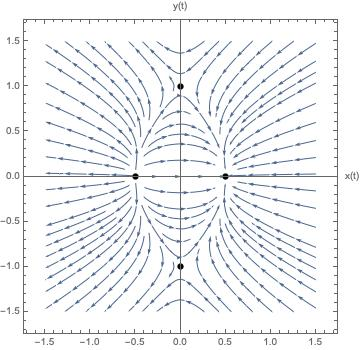
\includegraphics[width=.8\linewidth]{./HW6PhasePortrait.jpeg}
      \caption*{StreamPlot[\{$2 - 8 x^2 - 2 y^2$, $-6 x y$\}, \{x, -1.5, 1.5\}, \{y, -1.5, 1.5\}]}
    \end{figure}
    \end{flushleft}
\end{enumerate}
\end{enumerate}
\end{document}